\documentclass[12pt]{report}
\usepackage[a4paper,width=150mm,top=25mm,bottom=25mm,left=30mm,right=25mm,bindingoffset=6mm]{geometry}
\usepackage[utf8]{inputenc}
\usepackage{graphicx}
\usepackage{cite}
\usepackage{amsmath}
\usepackage{subcaption}
\usepackage{float}
\graphicspath{ {images/} }
\usepackage[bottom]{footmisc}
\usepackage{fixltx2e}
\usepackage{hyperref}
\usepackage{url}
\usepackage[demo]{graphicx}
\usepackage{subfig}
\usepackage{amsmath}
\usepackage{hyperref}
\usepackage[nottoc]{tocbibind}
\renewcommand{\bibname}{References}
\usepackage[titletoc]{appendix}
\documentclass{article}
\usepackage[table]{xcolor}
 
\setlength{\arrayrulewidth}{1mm}
\setlength{\tabcolsep}{18pt}
\renewcommand{\arraystretch}{2.5}

\linespread{1.25}

 
\title{
    {\textbf{A Study on Salient Region Detection Using Boundary and Color Cue}}\\
	{\large Department of Computer Science & Engineering,}\\
	{\large Khulna University of Engineering & Technology, Bangladesh}\\
	{\small \textbf{Report written by}}\\
	{\small Md Mosharaf Hossan, Roll:1307053}\\
	{\small Tushar Ghosh, Roll:1307060}\\
	{\small \textbf{Supervised by}}\\
	{\small Prof. Dr. Sk. Mohammad Masudul Ahsan}\\
    {\date{Feb 2018}}
}

\begin{document}

\maketitle
% * <mosharafkuet@gmail.com> 2018-02-10T09:09:26.388Z:
%
% ^.
% * <mosharafkuet@gmail.com> 2018-02-10T09:09:24.761Z:
%
%

\addtocontents{toc}{~\hfill\textbf{Page}\par}
\pagenumbering{roman}
\maketitle

\newpage
\addcontentsline{toc}{chapter}{Acknowledgement}
\chapter*{Acknowledgement}

All the praise to the almighty Allah, whose blessing and mercy helped us to complete this thesis work well. After that, we humbly acknowledge the valuable advice, guidance and co-operation of Dr. Sk. Md. Masudul Ahsan, Professor, Department of Computer Science and Engineering, Khulna University of Engineering & Technology, under whose supervision this work was carried out. His intellectual advices, encouragement and guidance make us feel confident and inspire to go through different research ideas. From him, we have learned that scientific research needs much effort in learning and applying and need to have a broad view at problems from different perspective. We would like to convey our heartiest gratitude to all the faculty members, officials and staffs of the Department of Computer Science and Engineering as they have always extended their co-operation to complete this work. Last but not least, we wish to thank our friends and family members for their constant support.

\newpage
\addcontentsline{toc}{chapter}{Abstract}
\chapter*{Abstract}
Detection of visually salient image regions is useful for
applications like object segmentation, adaptive compression,
and object recognition. In this thesis, we describe a novel approach of visually salient region detection from images based on color and spatial distribution. We assume that foreground objects are less likely to be positioned in the border and they have more color contrast with border regions. We also assume that salient region have relatively more contrast with it's surrounding regions than a nonsalient region. We use the information of color contrast to identify the salient region.Based on these two assumption we build global contrast map and boundary aware contrast map. We also assume that salient objects tend to cover relatively small area than nonsalient object. using this assumption we build another map called color importance map. then we combine these three maps to generate our final saliency map. Both qualitative and quantitative experiments are performed on a benchmark dataset which show that our approach performs well with other state of the art method.



\newpage
\addcontentsline{toc}{chapter}{Contents}

\tableofcontents

\listoffigures


\chapter{Introduction}
\pagenumbering{arabic}
\section{Introduction}

Many cognitive psychology researches have shown that given a visual scene, human attention is directed to particular parts by visual selective mechanism and these parts are called salient regions \cite{mangun1995neural}. In computer vision, salient region detection simulates the functionality of selective attention and localizes and tags the attention-grabbing regions or pixels in a digital image. Borji et al. \cite{borji2015salient} provided a more precise definition; they think that a salient region detection model should first detect the salient attention-grabbing objects in a context and then segment the whole objects. Usually, a generated saliency map is the output of the model and the intensity of each pixel in map means its probability of belonging to salient regions. According to this definition, we can know that this issue is essentially a figure/ground segmentation problem, and the goal is to only segment the salient foreground object from the background. However, it is slightly different from the traditional image segmentation problem that aims to partition an image into perceptually coherent regions.
Saliency detection for image is an important preprocessing step in many areas such as computer vision, graphics, and robotics to reduce computational cost by focusing on salient regions and neglecting the nonsalient. The value of salient region detection models lies on their wide applications, for instance, object detection and recognition \cite{ren2014region}, image and video compression \cite{guo2010novel}, thumb-nailing \cite{huang2011arcimboldo}, image quality assessment \cite{ li2013color}, image segmentation \cite{qin2014integration}, content based image retrieval \cite{feng2010attention}, and so on.



\noindent
Viewed from the information processing perspective, the existing models of visual saliency detection can be categorized as two main kinds: bottom-up and top-down. Bottom-up methods, also known as stimuli-driven or task-independent models, mainly detect saliency based on low-level feature attributes (color, orientation, motion, etc.) without any prior knowledge. Top-down approaches are often task-driven or scene-dependent models learning through training process, which requires some specific prior knowledge or high-level information. The human brains can perform this detection very quickly, and doing so on a computer remains a great challenge for researchers and scientists.


\section{Background}
The history of modern photography started many years back earlier in the 19th century. America’s history was filmed during the civil war with that in black and white. Many progressions have been made since then like digitization in photography.Kodak started to work on film-less technology in mid 70. At 1990 the commercial selling of digital cameras hits the road. The main benefit of storing the photographs in digital format is that these can be easily changed, reproduced and manipulated using different mathematic and computational algorithms. The Field of image processing is continually evolving. During the past five years, there has been a significant increase in the level of interest in image morphology, neural networks, full-color image processing, image data compression, image recognition, and knowledge-based image analysis systems. Image processing methods stems from two principal application areas: improvement of pictorial information for human interpretation, and processing of scene data for autonomous machine perception. Image is better than any other information form for our human being to perceive. 
\begin{figure}[here]%
    \centering
    \subfloat[Original image]{{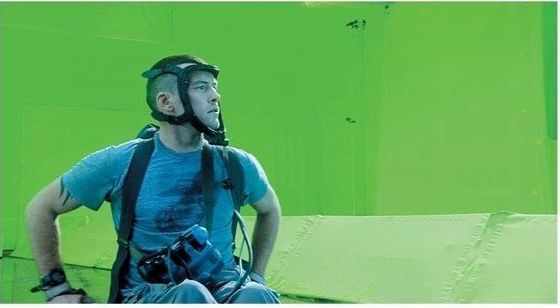
\includegraphics[width=0.45\textwidth,height=0.3\textwidth]{pictures/avatar1.jpg} }}%
    \qquad
    \subfloat[after processing]{{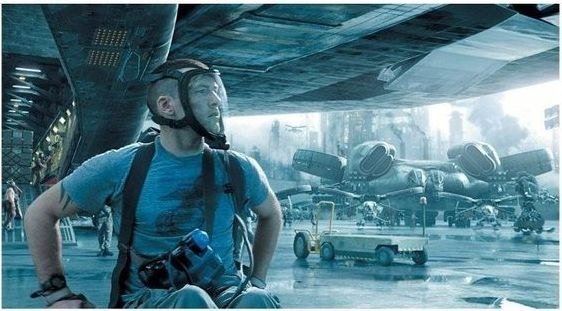
\includegraphics[width=0.45\textwidth,height=0.3\textwidth]{pictures/avatar2.jpg} }}%
    \caption{Applications of Background and Foreground Segregation in Movies \protect\footnotemark}%
    \label{superpixel}%
\end{figure}
 \footnotetext{https://i.pinimg.com/564x/da/5c/b4/da5cb4e048759581f48f145ded236ca6.jpg}
Vision allows humans to perceive and understand the world surrounding us. Image understanding, image analysis, and computer vision aim to duplicate the effect of human vision by electronically (= digitally, in the present context) perceiving and understanding image(s)In digital image processing system, first step in the process is Image Acquisition it require acquiring an image, After a digital image has been obtained, the next step deals with Preprocessing its function is to improve the image in ways that increase the chance for success of the other processes, the next step deals with Segmentation it partitions an input image into its constituent parts or objects, Representation & Description deals with make data in the form that suitable for computer processing, and after that Recognition is that assigns a label to an object, and last Interpretation involves meaning to an assemble of recognized objects.

This thesis work focuses on one important problem in computational photography namely visually salient region detection. It is a primary job that needs to be done smoothly before doing most of the other digital image processing related job. With the rapid increase in technology involved with images, need for detection of visually salient region efficiently is also increasing.For example We know that movies, dramas and other entertaining videos happens to contain amazing stuffs and stunts like acting on the space or in big ship in an ocean. Even though they seem impossible to film in there, they seem so realistic. How do they do that? Well, there’s a little trick in there. It’s not that they’re acted in that scene. Rather, that background of that scene was added by segregating background from the salient region and other post processing. 


 



\section{Problem statement}
There are many existing systems for visually salient region detection. Most researches related to visual attention are driven by local or global contrast on low-level stimulus, such as intensity, color, and orientation.
A common technique is to compare each regions color difference with other regions of the image and the region having more color difference than other regions are more likely to be the attention region.
some research also focuses on the spacial distribution of regions. These researches assume that the salient region are more likely to be on the center of the image than being the regions that touches the boundary.
As visually salient region detection which consists of foreground extraction and background subtraction is a far from perfect art, there are several problems one needs to take into account when developing visually salient region detection algorithms. The following common problems are:

\subsection{Camouflage}
When a foreground object has the same texture or color characteristics as the background, allowing the object to blend into the background.In that case if we compare a salient regions color with background region it doesn't give significant color difference so that we can identify that salient region  

\begin{figure}[here]
  \centering
  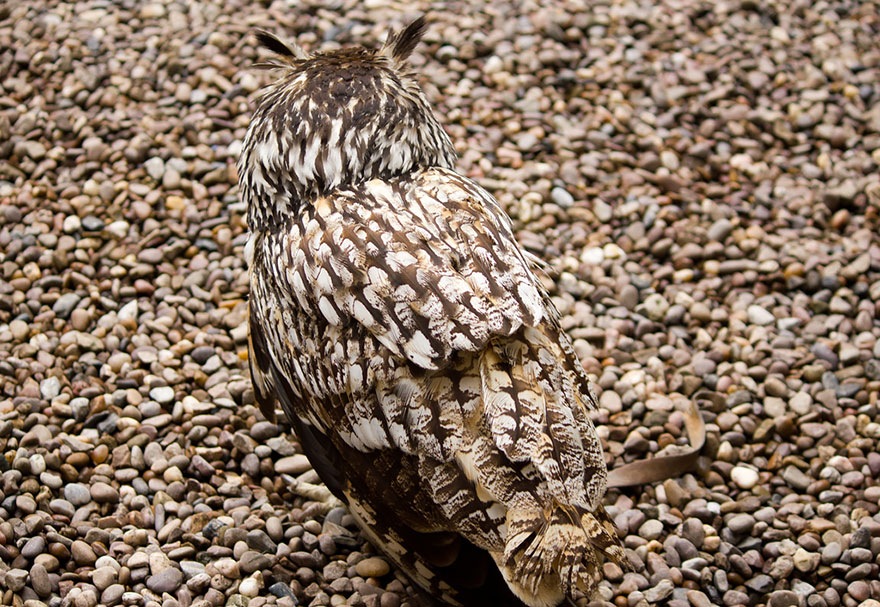
\includegraphics[width=0.55\textwidth,height=0.5\textwidth]{pictures/owl.jpg}
  \caption{Camouflage problem \protect\footnotemark}
  
  \label{orangeleaf}

\end{figure}
 \footnotetext{http://www.wikilinks.fr/wp-content/uploads/2013/06/camouflage-mimetisme-animal-camouflage-5.jpg}
 
\subsection{Partial matching color}
If part of a foreground object has same color as background,then differentiating full part of foreground with background becomes tough.


 
 
\begin{figure}[here]
  \centering
  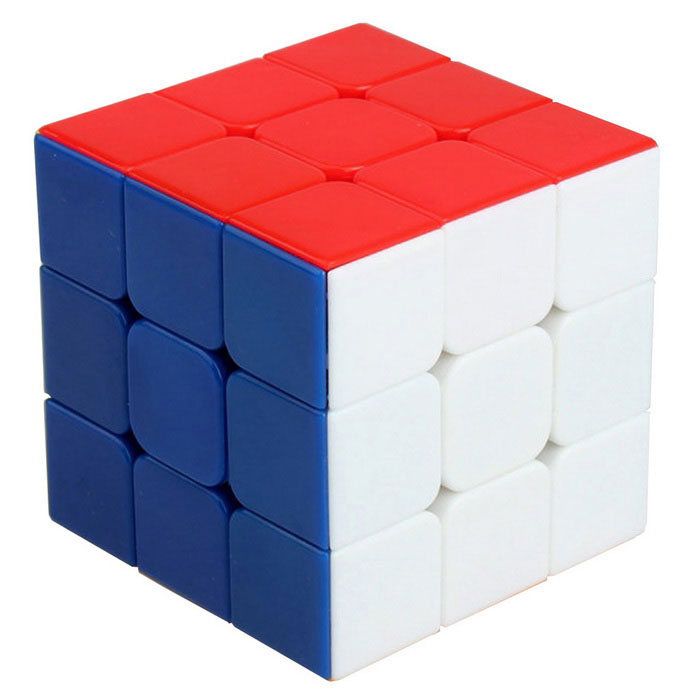
\includegraphics[width=0.55\textwidth,height=0.5\textwidth]{pictures/rubik.jpg}
  
  \caption{partial matching color problem \protect\footnotemark}
  
  \label{partial matching color}

\end{figure} 


 \footnotetext{http://img.dxcdn.com/productimages/sku_431118_1.jpg}

\subsection{Framed boundary}
If the boundary regions have frame with same color as foreground object then it becomes a difficult task to extract the salient region from it.

\begin{figure}[here]
  \centering
  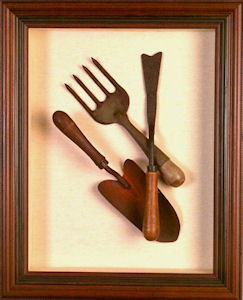
\includegraphics[width=0.35\textwidth,height=0.5\textwidth]{pictures/fork.jpg}
  
  \caption{partial matching color problem \protect\footnotemark}
  
  \label{partial matching color}

\end{figure} 

 \footnotetext{https://www.starvingartistframing.com/s/cc_images/cache_2850894204.jpg?t=1285712335}

\section{Motivation}
Saliency detection is an important preprocessing step in many application fields such as computer vision, robotics, and graphics. It reduces huge amount of computational cost by focusing on significant positions and neglecting the nonsignificant in the scene. So Most fields success depends on successful extraction of salient region from images. As human if we want to interact with the world then our eye becomes one of the most important part of our body. So in automated systems where we want to make the computer do humans job, we have to build something that acts as eye for the computer. using that eye computer will be able to see and understand things and make further decisions. As we know our brain tends to catch only the important region and ignore other regions surrounding it. It serves many purpose like understanding the situation faster and eliminating unnecessary computations and keep focus on the salient region. If we can simulate this wonderful characteristic of our eye and brain into a computer then it's going to be very helpful in real life applications of computers. For example for automated cars, drones and other unmanned vehicles faster scene analysis is a key requirement. visually salient region detection serves this purpose to simulate this wonderful characteristic of human eye for computer.

\section{Objectives}
The basic objective of this thesis is to make a robust system that can automatically detect and extract visually salient region from images
There is not any absolute system that can do this in complete manner. The main objectives of this thesis work are:
\begin{itemize}
  \item A detailed study on detection and extraction of visually salient region from images.
  \item To give a new idea on salient region detection.
  \item Implement and analyze performance on the proposed scheme based on accuracy, precision and recall.
\end{itemize}


 
\section{Organization of the thesis}
The rest of the thesis is organized as follows:
\begin{itemize}
  \item Chapter 2: This chapter discusses the literature surveys that have been done during this thesis. It also provides detailed survey of the literature related to visual saliency. Discussion about the existing and some new methods for salient region detection are done. This chapter presents the methodology and implementation of some existing and experimental results subsequently.
  \item Chapter 3: A new scheme for foreground extraction is proposed in here which uses color and spatial information of each region. A detailed study on visual saliency with our approach is discussed in here
  
  \item Chapter 4:The experimental outcomes of our proposed method along with necessary figures are discussed in details in this Chapter.
  \item Chapter 5:Recommendation for the future researchers of this work on the proposed model and the conclusive words about the model are outlined in this chapter.
  
\end{itemize}


 

  
\section{Conclusion}
In this chapter, we presented some background of digital image processing and a brief introduction of techniques for visually salient region detection.this chapter also discusses the basic objective of this thesis and the problems that needed to be taken into account when developing this algorithm

\chapter{Literature Review}
\section{Introduction}

With the rapid increase in technology involved in images, there is great needs to establish efficient  algorithms for what is known as salience detection, that is,finding regions or object of interest in an image.The human brains can perform this detection very quickly, and doing so on a computer is a great task for researchers and scientists.This problem is related to image cropping, object recognition and image cropping.Mostly researchers divide this problem into two category.One is global scheme and local scheme.In local scheme a salient region is calculated with respect to it's local region in an image whereas global scheme give priority to when a region is distinct with respect to the whole region of an image.There are some other methods where researcher combined these global and local scheme to get salient region of an image.

\subsection{Local and Global Approaches}
Bottom-up approaches focuses on cues that we naturally interested in, like colors, orientation, density and frequency  

\begin{description}
  \item[$\bullet$]Itti, Koch and Niebur\cite{itti1998model}   proposed a visual attention
  model in which image features such as color, intensity, and
orientation for LDR images are combined to form a single saliency map.It makes use of Gaussian based approach in
which a Gaussian pyramid is formed in each channel by subsampling the input image.Each feature is computed by a set of linear centre-surround operations. Centre-surround is implemented in the model as the difference between fine and coarse scales. The across-scale subtraction is obtained by interpolation to the centre scale and point-by-point
subtraction. Afterwards, all feature maps are combined into a “conspicuitymap” in each channel. Conspicuity maps from all channels one master saliency map, which topographically represents the local saliency.


\item[$\bullet$] Sidib{\'e}, D{\'e}sir{\'e} and M{\'e}riaudeau\cite{sidibe2016visual}  proposed saliency  based on the common observation
that local salient regions exhibit distinct geometric and texture patterns
from neighbouring regions. The colour distribution of local image
patches is modelled with a Gaussian density and measure the saliency
of each patch as the statistical distance from that density.


\begin{figure}[h!]
  \centering
  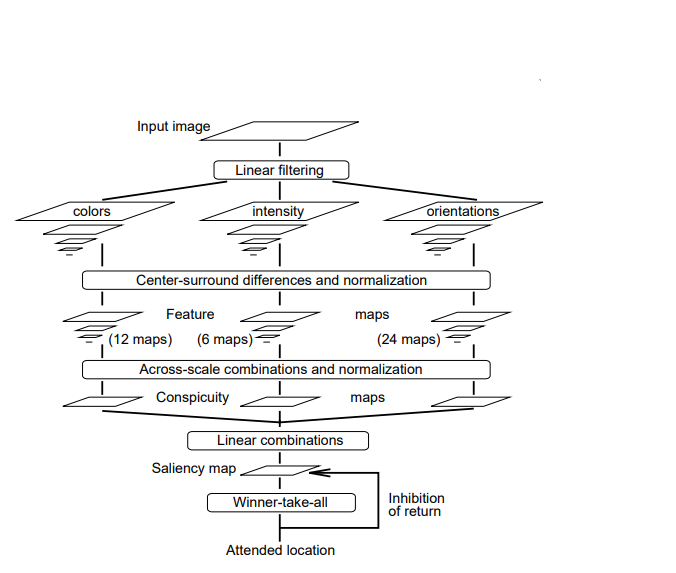
\includegraphics[width=1\textwidth,height=1\textwidth]{pictures/figure1.png}
  \caption[]{Framework of visual attention for Rapid Scene Analysis \cite{itti1998model}}
  \label{orangeleaf}

\end{figure}

\item[$\bullet$]Nevrez mamolu, Weisi Lin, and Yuming Fang \cite{imamoglu2013saliency} 
suggested a saliency detection model in which image is
represented as quaternionic and developed a multiresolution
spatiotemporal saliency detection model called phase
spectrum of quaternion Fourier transform (PQFT) to compute
the spatiotemporal saliency map from the images quaternion
representation. First, each pixel of the image is represented by
a quaternion that consists of color, intensity and motion
feature. Then, the phase spectrum of QFT is used to calculate
the spatiotemporal saliency map, which considers not only
salient spatial features like color, orientation and others in a
single frame but also temporal feature between frames like
motion.

\item[$\bullet$] Qinmu Peng, Yiu-ming Cheung and Xingeand Yuan \cite{peng2017hybrid} , presents a visual saliency detection approach,
which is a hybrid of local feature-based saliency and global
feature-based saliency. First, for a given input image, use an
automatic selection of smoothing parameter scheme to make
the image region more homogeneous. Then, partition the
smoothed image into a set of regions and compute the local
saliency by measuring the color and texture dissimilarity in
the smoothed regions and the original regions, respectively.
Furthermore, compute the global saliency by utilizing the
global color distribution model embedded with color
coherence, together with the multiple edge saliency. Finally,
combine the local and global saliencies, and utilize the
composition information to obtain the final saliency

\begin{figure}[h!]
  \centering
  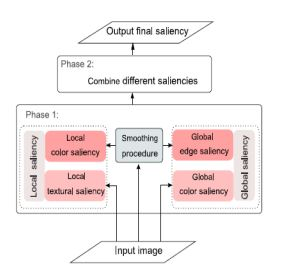
\includegraphics[width=.5\textwidth,height=.6\textwidth]{pictures/figure2.JPG}
  \caption[]{Hybrid of local and global saliency detection\cite{peng2017hybrid}}
  \label{orangeleaf}

\end{figure}


\item[$\bullet$] Yan and Zhi chun \cite{ren2014salient}  presents visual saliency detects which is based on fast bottom-up data driven saliency detection using global contrast method which extracts a large-scale object from background.The global contast based method uniformly
highlighting entire objects is preferred over local contast
based methods which produce high saliency values at or
near object edges. The region based texture contrast is
incorporated into the process of salient map computation
upon the basis of the region based color contrast

\item[$\bullet$] Zhixiang Ren, Shenghua Gao, Liang-Tien Chia\cite{ren2014region}, and
Ivor Wai-Hung Tsang presents a region-based solution for
saliency detection applicable to better encode the image
features for solving object recognition task. First use the
adaptive mean shift algorithm to extract superpixels from the
input image. Then apply Gaussian mixture model (GMM) to
cluster superpixels based on their color similarity. Finally,
calculate the saliency value for each cluster using spatial
compactness metric together with modified PageRank
propagation.

\begin{figure}[h!]
  \centering
  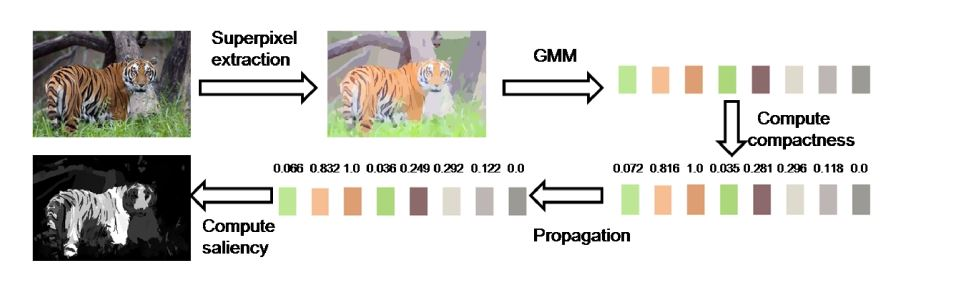
\includegraphics[width=1\textwidth,height=.5\textwidth]{pictures/figure3.jpg}
  \caption[]{Region-Based Saliency Detection\cite{ren2014region}}
  \label{orangeleaf}
\end{figure}

\item[$\bullet$] Zhu, Shuang, Yichen \cite{zhu2014saliency}  propose a robust back-ground measure
called background connectivity.It characterizes the spatial layout of image regions with respect to
image boundaries and is much more robust. It has an intuitive geometrical interpretation and presents unique benefits that are absent in previous saliency measures.Then they propose a principle optimization framework to intregate multiple low level cues including background measure to obtain clean and uniform saliency maps.



\item[$\bullet$] Achanta,R,Hermani\cite{achanta2009frequency}  proposed introduced a frequency tuned saliency detection method. Using the color
differences from the average image color to define pixel saliency.

\item[$\bullet$] Chenlei Guo and Liming Zhang \cite{guo2010novel}  presents a saliency
detection model based on high-pass coefficients of the
wavelet decomposition. The idea is to create the feature maps
by IWT on the multi-level decomposition. First, RGB image
is converted into LAB color space. Then, apply wavelet
transform decomposition on the noise removed version to find
scaling coefficients. In addition to it, it focuses on creating the
feature maps by IWT on the multi-level decomposition. Two
saliency maps are created: local and global saliency maps.
Finally, the local and global maps are combined to yield the
final saliency map. The final saliency map represents both the
local contrast of each location on the scene and the global
distribution of the features as an amplifier for local saliency
values

\item[$\bullet$] Zhi Liu, Xiang Zhang, Shuhua Luo, and Olivier\cite{liu2014superpixel}  proposed a superpixel-based spatiotemporal saliency
model for saliency detection in videos. First, based on the
superpixel representation of video frames, motion histograms
and color histograms are extracted at the superpixel level as
local features and frame level as global features. Then,
superpixel level temporal saliency is measured by integrating
motion distinctiveness of superpixels with a scheme of
temporal saliency prediction and adjustment, and superpixellevel spatial saliency is measured by evaluating global
contrast and spatial sparsity of superpixels. Finally, a pixellevel saliency derivation method is used to generate pixellevel temporal and spatial saliency maps, and an adaptive
fusion method is exploited to integrate them into the
spatiotemporal saliency map.

\begin{figure}[h!]
  \centering
  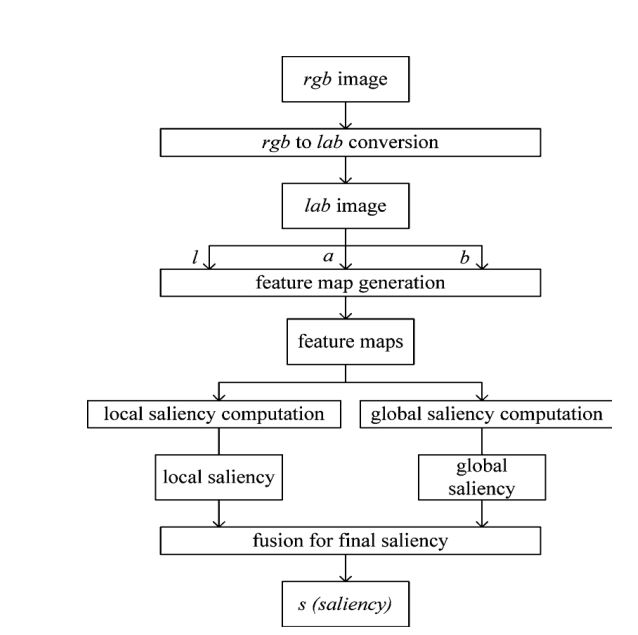
\includegraphics[width=1\textwidth,height=0.9\textwidth]{pictures/figure4.jpg}
  \caption[]{Framework of visual attention for Rapid Scene Analysis \cite{guo2010novel}}
  \label{orangeleaf}
\end{figure}

\item[$\bullet$] Yuanyuan Dong, Mahsa T. Pourazad, and Panos
Nasiopoulos\cite{dong2016human}   proposed a saliency detection method that
detects the saliency of HDR images and HDR video frames.
The spatial and temporal cues are taken into account, leading
to two saliency maps: the spatial saliency map and the
temporal saliency map. First, to obtain the spatial saliency
map, use the HVS model to decompose feature channels from
an HDR input and then follow the procedure of the classical
bottom-up method in \cite{itti1998model}. Then to compute the temporal
saliency map, an optical flow based method is used to
estimate motion. Finally, a dynamic fusion method is
proposed to combine both the spatial and temporal saliency
maps.

\item[$\bullet$]Libio ,Lin and Tiejian \cite{zhang2016unified}  proposed visual saliency based on 
color and texture features and incorporating higher-level priors.The SLIC superpixel algorithm is applied to form an over-segmentation of the image. Color saliency map and texture
saliency map are calculated based on the region contrast method and adaptive weight.
Higher-level priors including location prior and color prior are incorporated into the model to
achieve a better performance and full resolution saliency map is obtained by using the upsampling method. 

\item[$\bullet$] M.M. Cheng et al. \cite{cheng2015global}  presented a regional contrast
based salient object detection algorithm that evaluated global contrast differences and spatial
weighted coherence scores. They used the saliency maps to accomplish unsupervised salient
object segmentation.



\item[$\bullet$] Wonjun Kim, Chanho Jung, and Changick Kim \cite{kim2011spatiotemporal} 
suggested a novel unified method for detecting salient regions
in both images and videos based on a discriminant centersurround hypothesis that the salient region stands out from its
surroundings. First of all, a set of visual features composed of
edge and color orientations and temporal gradients are
computed. Then, compute the spatiotemporal saliency at each
scale in which the spatial saliency is computed as the
distances between ordinal signatures of edge and color
orientations obtained from the center and the surrounding
regions and the temporal saliency, by simply computing the
sum of absolute difference (SAD) between temporal gradients
of the center and the surrounding regions. Finally, resize
saliency map to the same size of input image to obtain the
final saliency.


\end{description}

\section{Conclusion}
In this chapter, we presented the common method for finding visual saliency detection.By previewing various method we learned advantage and disadvantage of various method and their characterstic
for simple and clean visual saliency detection.

\chapter{Visual and Color Saliency}
\section{Introduction}

Visual salience (or visual saliency) is the distinct subjective perceptual quality which makes some items in the world stand out from their neighbors and immediately grab our attention.
Our attention is attracted to visually salient stimuli. It is important for complex biological systems to rapidly detect potential prey, predators, or mates in a cluttered visual world. However, simultaneously identifying any and all interesting targets in one's visual field has prohibitive computational complexity making it a daunting task even for the most sophisticated biological brains (Tsotsos, 1991), let alone for any existing computer. One solution, adopted by primates and many other animals, is to restrict complex object recognition process to a small area or a few objects at any one time. The many objects or areas in the visual scene can then be processed one after the other. This serialization of visual scene analysis is operationalized through mechanisms of visual attention: A common (although somewhat inaccurate) metaphor for attention is that of a virtual spotlight, shifting to and highlighting different sub-regions of the visual world, so that one region at a time can be subjected to more detailed visual analysis (Treisman & Gelade, 1980; Crick, 1984; Weichselgartner & Sperling, 1987).
\noindent
Visual attention may be a solution to the inability to fully process all locations in parallel. However, this solution produces a problem. If you are only going to process one region or object at a time, how do you select that target of attention? Visual salience helps your brain achieve reasonably efficient selection. Early stages of visual processing give rise to a distinct subjective perceptual quality which makes some stimuli stand out from among other items or locations. Our brain has evolved to rapidly compute salience in an automatic manner and in real-time over the entire visual field. Visual attention is then attracted towards salient visual locations.
The core of visual salience is a bottom-up, stimulus-driven signal that announces “this location is sufficiently different from its surroundings to be worthy of your attention”. This bottom-up deployment of attention towards salient locations can be strongly modulated or even sometimes overridden by top-down, user-driven factors (Desimone & Duncan, 1995; Itti & Koch, 2001). Thus, a lone red object in a green field will be salient and will attract attention in a bottom-up manner (see illustration below). In addition, if you are looking through a child’s toy bin for a red plastic dragon, amidst plastic objects of many vivid colors, no one color may be especially salient until your top-down desire to find the red object renders all red objects, whether dragons or not, more salient.
Visual salience is sometimes carelessly described as a physical property of a visual stimulus. It is important to remember that salience is the consequence of an interaction of a stimulus with other stimuli, as well as with a visual system (biological or artificial). As a straight-forward example, consider that a color-blind person will have a dramatically different experience of visual salience than a person with normal color vision, even when both look at exactly the same physical scene (see, e.g., the first example image below). As a more controversial example, it may be that expertise changes the salience of some stimuli for some observers. Nevertheless, because visual salience arises from fairly low-level and stereotypical computations in the early stages of visual processing (details in the following section), the factors contributing to salience are generally quite comparable from one observer to the next, leading to similar experiences across a range of observers and of behavioral conditions.
\noindent
Visual Saliency is the distinct subjective perceptual quality which makes some items in the world or in a scene stands out from their neighbors and immediately grab our attention. Human brains can do this task very fast as it uses intuition.It is a saliency measure based on visual components of the source, such as color or spacial distribution. It tells how important a region is in an image which is done by comparing the region color and some other cues with other regions. By getting the measurement , we get the most salient regions and relatively less salient region. Then we mark the most salient regions as foreground and relatively less salient regions as background
To find visual saliency, the Image is subdivided into small regions.  It is done because it requires high computation time to compare each pixel of image with all other pixels. For example, if an image consists 400x600 pixels then for computation, the need to compare total (400x600)x(400x600 − 1) pixels or 57504000000 comparisons which might require a lot of time to process each frame. Rather doing so many comparisons, the image first is segmented into small regions. In this approach the work is done which an approach called SLIC\cite{achanta2012slic}.  This method subdivides the whole image into some small regions which are called Superpixels. Superpixels are generally have a fixed size in area, but not fixed in shape.



\section{Image Segmentation using SLIC}

At first an image is segmented into number of (N) homogeneous super-pixels using the SLIC algorithm\cite{achanta2012slic}. SLIC or Simple Linear Iterative Clustering is a segmentation method that segments an image into small regions. Each of these superpixels is considered as a region . In each region every pixels will get the same color . This color will be the average color calculated from each pixels in a region rather than every pixel, we calculate saliency for a region. The color and spatial features of a superpixel are defined as the mean of all the pixels comprising the superpixel in the CIELab color space and image. SLIC adapts k-means clustering approach to efficiently generate superpixels. It also adheres to boundaries as well as other faster and efficient in memory management.
The main purpose of using SLIC is to reduce computation cost. For example 
if we segment an image having dimensions 400x600 pixels into 200 superpixels then the number of comparison reduces from 57504000000 to 200x199 or 39800.So we can see that the computation cost is significantly reduced. SlIC is a straight forward extend to supervoxel generation.

\begin{figure}[here]%
    \centering
    \subfloat[Original image]{{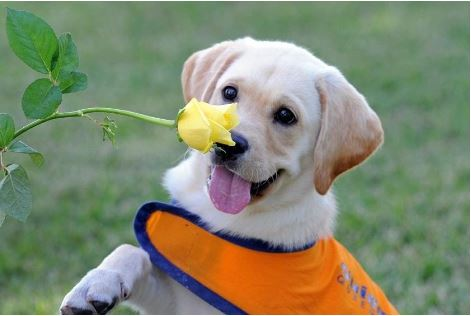
\includegraphics[width=0.45\textwidth,height=0.3\textwidth]{pictures/slic1.jpg} }}%
    \qquad
    \subfloat[Calculated Superpixel Boundaries]{{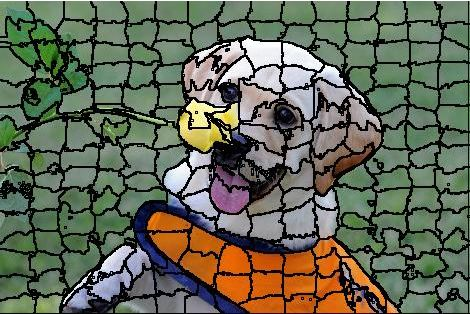
\includegraphics[width=0.45\textwidth,height=0.3\textwidth]{pictures/slic2.jpg} }}%
    
    \subfloat[Recolored image]{{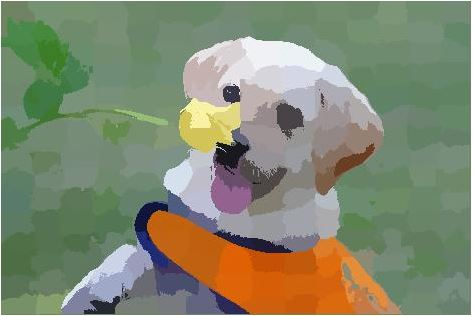
\includegraphics[width=0.45\textwidth,height=0.3\textwidth]{pictures/slic3.jpg} }}%
    
    \caption{Original image and segmented image}%
    \label{superpixel}%
\end{figure}
\noindent
In the segmented image, each region is identified by a boundary as shown. Here each region is shown with a single color rather than the color of all pixels. This single color can be found by calculating mean of the all pixels of that region. This color is used as a substitute of all colors of that region.


\section{Finding Global Contrast Map}
 We use the most widely used prior, i.e., the contrast prior ,which means that the color components belonging to a salient object often have strong contrast to their surroundings. Similarity  between two regions r\textsubscript{i},r\textsubscript{j},\textit{i,j=1.2.....N} is calculated by equation \eqref{1}. where ci and cj are the average color vector of the regions in LAB color space, σ is a constant which controls the strength of the weight and d is a distance function which calculates color based similarity between regions.
 
 \begin{equation}\label{1}
d\textsubscript{c}(r\textsubscript{i},r\textsubscript{j})&= e^{-\frac{||c\tectsubscript{i}-c\textsubscript{j}||^2}{\sigma^2}}
\end{equation}
\noindent
 But color dissimilarity is our main concern. So for this purpose we use equation \eqref{2}.
 
 \begin{equation}\label{2}
\rho \textsubscript{c}(r\textsubscript{i},r\textsubscript{j}) &= 1- d\textsubscript{c}(r\textsubscript{i},r\textsubscript{j}) 
\end{equation}
\noindent
 For every region r\textsubscript{i} This value from equation \eqref{2} is then averaged with every other superpixels of the image to get color priori based rarity of region r\textsubscript{i} Using equation \eqref{3}. 
 
 \begin{equation}\label{3}
s\textsubscript{c}(r\textsubscript{i}) &= \frac{1}{N} \sum_{k=1}^{N} \rho \textsubscript{c}(r\textsubscript{i},r\textsubscript{k})
\end{equation}

\begin{figure}[here]%
    \centering
    \subfloat[Original image]{{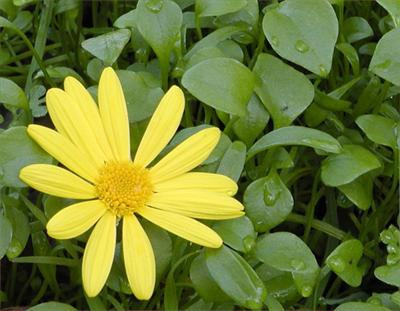
\includegraphics[width=0.45\textwidth,height=0.3\textwidth]{pictures/10841/color_image.jpg} }}%
    \qquad
    \subfloat[Global Contrast Map]{{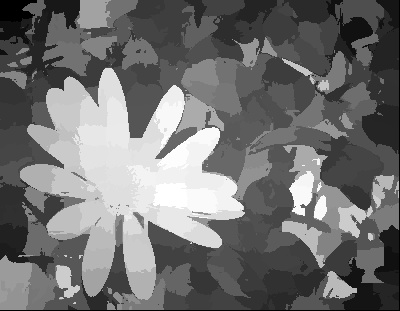
\includegraphics[width=0.45\textwidth,height=0.3\textwidth]{pictures/10841/globalsaliencyMap.jpg} }}%
    \caption{generated global contrast map}%
    \label{superpixel}%
\end{figure}
 \noindent
 image region with similar colors are likely to have the same label . However, this can produce false alarms when part of the background has a similar color to the foreground object. Therefore, we incorporate the spatial distance d\textsubscript{s} between regions normalized by the image size to down-weight the importance of distant regions according to the assumptions in Table 1\cite{masudsir2016}.
 We calculate d\textsubscript{s} by using equation \eqref{4} Where p\textsubscript{i} and p\textsubscript{j} are the average position vector of the regions r\textsubscript{i} and r\textsubscript{j} respectively. Equation \ref{5} defines the dissimilarity between two region r\textsubscript{i},r\textsubscript{j} including both color and spatial prior, where $\gamma$ is a constant used to avoid the division by zero and defined by equation \eqref{6}
 
\begin{equation}\label{4}
d\textsubscript{s}(r\textsubscript{i},r\textsubscript{j})&= ||p\textsubscript{i}-p\textsubscript{j}||^2
\end{equation}

\begin{equation}\label{5}
\rho \textsubscript{c,s}(r\textsubscript{i},r\textsubscript{j})&=  \frac{\rho\textsubscript{c}(r\textsubscript{i},r\textsubscript{j})}{d\textsubscript{s}(r\textsubscript{i},r\textsubscript{j})+\gamma}
\end{equation}
 
 
\begin{equation}\label{6}
\gamma &= 1-e^\frac{1}{\sigma^2}
\end{equation}
\noindent
and finally equation \eqref{6} gives the global saliency value of a region r\textsubscript{i} after comparing it with all other regions of the image. Fig. 3.2(b) shows the global contrast map\cite{masudsir2016} of the Fig. 1(a) generated by equation \ref{6}.









\begin{equation}\label{7}
S\textsubscript{G}(r\textsubscript{i}) &= \frac{1}{N} \sum_{k=1}^{N} \rho \textsubscript{c,s}(r\textsubscript{i},r\textsubscript{k})
\end{equation}





 
{\rowcolors{3}{green!80!yellow!50}{green!70!yellow!40}

\begin{tabular}{ |p{3cm}|p{3cm}|p{3cm}|  }
\hline
\multicolumn{3}{|c|}{Table 1: Saliency proportionality for color and distance} \\
\hline
Color Distance & Spatial Distance & Saliency \\
\hline
Low & Near & Low  \\
Low & Far   & Low  \\
High & Near & High  \\
High & Far & X \\
\hline
\end{tabular}
}

\section{Boundary Aware Contrast Map}
Global contrast map works nicely if  the background is more simple smooth . but when the background will be complex global contrast priori can not eliminate background fully .To solve this  problem boundary awareness\cite{masudsir2016} is needed where each region is compared with other regions that touches the boundary to find the difference of color. Let's consider there are M number of regions that touches the border. We take every region r\textsubscript{i}  and compare it's color difference with those M regions and store the value in a vector. equation \eqref{8} is used to do this job.here r\textsubscript{i} denotes each region b\textsubscript{j} denotes the regions that touches border. $\rho$\textsubscript{c,s} denotes the color and spatial dissimilarity between each region and boundary regions. 

\begin{equation}\label{8}
B\textsubscript{i}[j] &= \rho\textsubscript{c,s}(r\textsubscript{i},b\textsubscript{j})
\end{equation}


\noindent
Data after the calculation is stored in B\textsubscript{i} which is the color dissimilarity vector.this vector is then sorted in ascending order using equatio \eqref{9}.

\begin{equation}\label{9}
B\textsubscript{i} &= sort(B\textsubscript{i})
\end{equation}
\noindent
we sort the vector so that the small values (that represents less difference in color) stays in front of the vector and thereby it becomes easier to select the desired
range of values. Finally, the boundary aware saliency value of r\textsubscript{i} is assigned by using equation \eqref{10}, where 0 <$\alpha$< 1. By equation \eqref{10}, we are actually taking the average of $\alpha$M minimal dissimilarity (i.e., to some extent similar) values with the assumption that a region similar to the boundary regions will generally produce a very lower measure and thereby suppress the background regions.


\begin{figure}%
    \centering
    \subfloat[Global Contrast Map]{{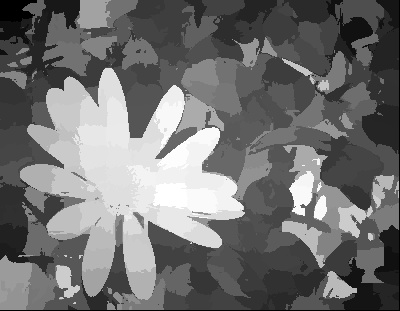
\includegraphics[width=0.45\textwidth,height=0.3\textwidth]{pictures/10841/globalsaliencyMap.jpg} }}%
    \qquad
    \subfloat[Bondary Aware Contrast Map]{{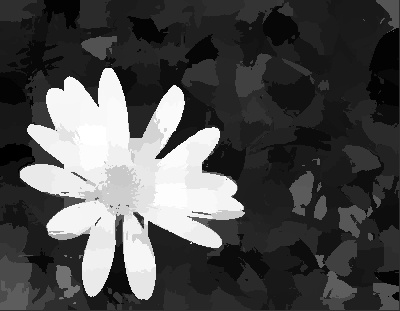
\includegraphics[width=0.45\textwidth,height=0.3\textwidth]{pictures/10841/BoundarysaliencyMap.jpg} }}%
    \caption{generated boundary aware contrast map}%
    \label{superpixel}%
\end{figure}
 


\begin{equation}\label{10}
S\textsubscript{B}(r\textsubscript{i}) &=\frac{1}{\alpha M} \sum_{k=1}^{\alpha M} B\textsubscript{i}k
\end{equation}

\noindent
For example if we consider 4 regions that touches the border and we want to calculate the value of region r\textsubscript{i} then using equation \eqref{8} we will get four values. Say those values are 0.45,0.37,0.52,0.63. after applying equation \eqref{9} the color dissimilarity vector will have 0.37,0.45,0.52,0.63 in ascending order. Now if we consider $\alpha$ = 0.5 then first two item will be chosen and and the average of those will be 0.41 and if we consider another region which after following the same procedure gives 0.21 as output then we can assume that the first region with value 0.41 is more salient than the region with value 0.21







\section{Color Saliency}

Color saliency of an image is defined by distinctness of color in an image. The more the region have more distinct color it is considered as more salient that means more the probability of being foreground and the region which have less distinct color it is considered as less salient and as a result more probability of being background. In this thesis we proposed a simple method for finding color saliency of an image. To get the distinct color we take the difference of mean color from the image as a result a region having low color frequency can be found.

\subsection{Lab Color Space}
The Lab color space describes mathematically all perceivable colors in the three dimensions L for lightness and a and b for the color components green–red and blue–yellow. The terminology "Lab" originates from the Hunter 1948 color space.[1][2] Nowadays "Lab" is frequently mis-used as abbreviation for CIEL*a*b* 1976 color space (also CIELAB); the asterisks/stars distinguish the CIE version from Hunter's original version. The difference from the Hunter Lab coordinates is that the CIELAB coordinates are created by a cube root transformation of the CIE XYZ color data, while the Hunter Lab coordinates are the result of a square root transformation. Other, less common examples of color spaces with Lab representations make use of the CIE 1994 color difference and the CIE 2000 color difference.The Lab color space exceeds the gamuts of the RGB and CMYK color models (for example, ProPhoto RGB includes about 90 percent all perceivable colors). One of the most important attributes of the Lab model is device independence. This means that the colors are defined independent of their nature of creation or the device they are displayed on. The Lab color space is used when graphics for print have to be converted from RGB to CMYK, as the Lab gamut includes both the RGB and CMYK gamut. Also it is used as an interchange format between different devices as for its device independence. The space itself is a three-dimensional real number space, that contains an infinite number of possible representations of colors. However, in practice, the space is usually mapped onto a three-dimensional integer space for device-independent digital representation, and for these reasons, the L*, a*, and b* values are usually absolute, with a pre-defined range. The lightness, L*, represents the darkest black at L* = 0, and the brightest white at L* = 100. The color channels, a* and b*, will represent true neutral gray values at a* = 0 and b* = 0. The red/green opponent colors are represented along the a* axis, with green at negative a* values and red at positive a* values. The yellow/blue opponent colors are represented along the b* axis, with blue at negative b* values and yellow at positive b* values. The scaling and limits of the a* and b* axes will depend on the specific implementation of Lab color, as described below, but they often run in the range of ±100 or −128 to +127 (signed 8-bit integer).

\subsection{Average Color Lab Image}
At first an image is converted into lab color image.Figure ~\ref{fig:conversion} shows the conversion from input to output image.Lab image has three channel and they are L-channel, a-channel, b-channel.Now mean, mode and average color is calculated separately for l-channel, a-channel and b-channel.Then global average color 
 C\textsubscript{avg} &= [L\textsubscript{avg},a\textsubscript{avg},b\textsubscript{avg}] in 
each channel is calculated from equation \ref{10}, \ref{11}, \ref{12}. 

\begin{equation}\label{10}
L\textsubscript{avg} &=min(\frac{(L\textsubscript{mean}+L\textsubscript{mode})}{2},L\textsubscript{mean})
\end{equation}

\begin{equation}\label{11}
a\textsubscript{avg} &=\frac{(a\textsubscript{mean}+a\textsubscript{mode})}{2}
\end{equation}

\begin{equation}\label{12}
b\textsubscript{avg} &=\frac{(b\textsubscript{mean}+b\textsubscript{mode})}{2}
\end{equation}


\begin{figure}[here]%
    \centering
    \subfloat[Input image]{{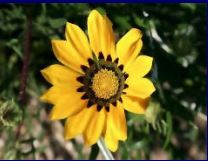
\includegraphics[width=0.45\textwidth,height=0.3\textwidth]{pictures/color_sal/1.jpg} }}%
    \qquad
    \subfloat[Lab image]{{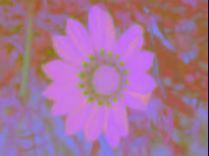
\includegraphics[width=0.45\textwidth,height=0.3\textwidth]{pictures/color_sal/2.jpg} }}%
    \caption{Conversion from input to lab image}%
    \label{fig:conversion}%
\end{figure}

\begin{figure}[here]%
    \centering
    \subfloat[l-channel]{{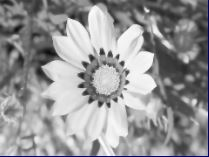
\includegraphics[width=0.45\textwidth,height=0.3\textwidth]{pictures/color_sal/3.jpg} }}%
    \qquad
    \subfloat[a-channel]{{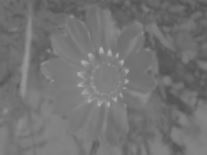
\includegraphics[width=0.45\textwidth,height=0.3\textwidth]{pictures/color_sal/4.jpg} }}%
    \qquad
    \subfloat[b-channel]{{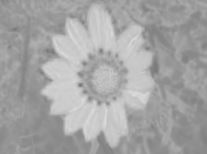
\includegraphics[width=0.45\textwidth,height=0.3\textwidth]{pictures/color_sal/5.jpg} }}%
    \caption{Different channel image in lab image}%
    \label{fig:conversion}%
\end{figure}

\subsection{Absolute Difference Lab Image}
Average color vector now used to compute absolute difference lab image.For each pixel having row x and column y 
absolute difference between that pixels intensity in three channel and average intensity in L-channel,a-channel and b-channel is calculated using equation \ref{13}

for L-channel
\begin{equation}\label{13}
DI\textsubscript{L}(x,y) &= |(I\textsubscript{L}(x,y) - L\textsubscript{avg})|
\end{equation}


for a-channel
\begin{equation}\label{14}
DI\textsubscript{a}(x,y) &= |(I\textsubscript{a}(x,y) - a\textsubscript{avg})|
\end{equation}


for b-channel
\begin{equation}\label{15}
DI\textsubscript{b}(x,y) &= |(I\textsubscript{b}(x,y) - b\textsubscript{avg})|
\end{equation}

Combing these three equation it can be written as vector equation \ref{16}


\begin{equation}\label{16}
DI\textsubscript{Lab}(x,y) &= |(I\textsubscript{Lab}(x,y) - C\textsubscript{avg})|
\end{equation}


\begin{figure}[here]%
    \centering
    \subfloat[Diff. Lab Image]{{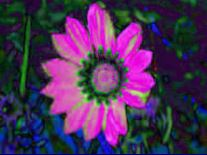
\includegraphics[width=0.45\textwidth,height=0.3\textwidth]{pictures/color_sal/6diff.jpg} }}%
    \qquad
    \subfloat[Diff. L-channel]{{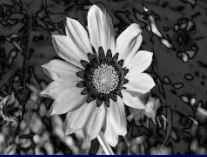
\includegraphics[width=0.45\textwidth,height=0.3\textwidth]{pictures/color_sal/diff3.jpg} }}%
    \qquad
    \subfloat[Diff. a-channel]{{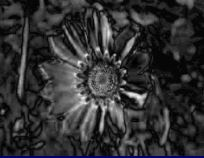
\includegraphics[width=0.45\textwidth,height=0.3\textwidth]{pictures/color_sal/diff4.jpg} }}%
    \qquad
    \subfloat[Diff. b-channel]{{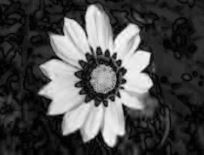
\includegraphics[width=0.45\textwidth,height=0.3\textwidth]{pictures/color_sal/diff5.jpg} }}%
    \caption{Absolute Difference lab image}%
    \label{fig:conversion}%
\end{figure}


\subsection{Color Map}
Final color map is the combination of three image. These three images are absolute difference L-channel, a-channel, b-channel images.
These three image are combined by weighted combination of their intensity values to get two images of single channel. Three channel image thus converted into single channel image using following equation  to get M,N 


\begin{equation}\label{17}
M\textsubscript{gray}(x,y) &= w\textsubscript{L}DI\textsubscript{L}(x,y) +w\textsubscript{a}DI\textsubscript{a}(x,y)+w\textsubscript{b}DI\textsubscript{b}(x,y) 
\end{equation}


\begin{equation}\label{18}
N\textsubscript{gray}(x,y) &= \sqrt{DI\textsubscript{L}^2(x,y)+DI\textsubscript{a}^2(x,y)+DI\textsubscript{b}^2(x,y)}
\end{equation}

here M is an image of single channel. Three channel L-channel,a-channel,b-channel are combined by weight w\textsubscript{L}, 
w\textsubscript{a} and w\textsubscript{b}. N is an single channel image combined by taking squared sum of three channel intensity values.
Final color Map is extracted by combining M and N image by equation \ref{20}

\begin{equation}\label{20}
MAP\textsubscript{color}(x,y) &= M^\gamma * N(x,y) 
\end{equation}
All the images are normalized after pixel level calculation. After getting median filter on MAP image it's saliency is calculated.


\subsection{Color Saliency Calculation}
Color saliency defines the most salient color of the image. If saliency is high then that pixel or region is most 
salient or foreground and if slaiency is low then that pixel or region is background or non-salient object. To find out the color saliency at first color map image is segmented by same number of region as original image. Then each region average value is calculated. Average intensity value is calculated by dividing sum of all pixels intensity in a region with the number of pexels in the region. Later saliency is calculated by dividing the average value by 255. Normalizing the value saliency will range from 0 to 1 for a region. Saliency value 1 means that region is most salient and its value 0 means that region is non salient.

\begin{figure}[t]%
    \centering
    \subfloat[N image]{{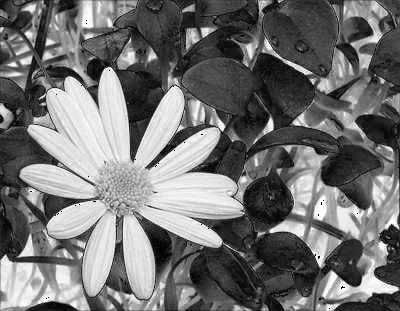
\includegraphics[width=0.3\textwidth,height=0.2\textwidth]{pictures/10841/N_xy.jpg} }}%
    \qquad
    \subfloat[M image]{{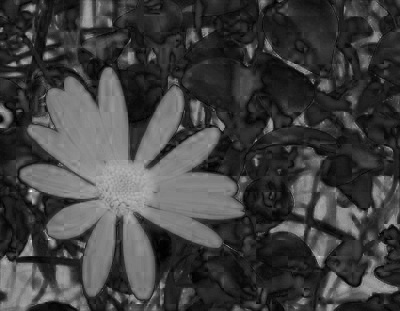
\includegraphics[width=0.3\textwidth,height=0.2\textwidth]{pictures/10841/g_xy.jpg} }}%
    \qquad
    \subfloat[Color Map]{{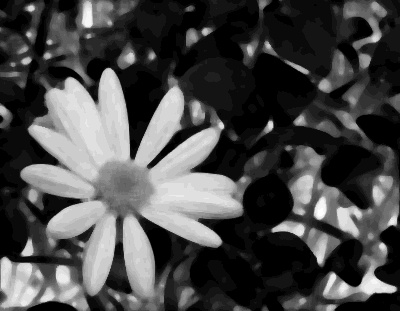
\includegraphics[width=0.3\textwidth,height=0.2\textwidth]{pictures/10841/median.jpg} }}%
    \qquad
    \subfloat[Color Saliency]{{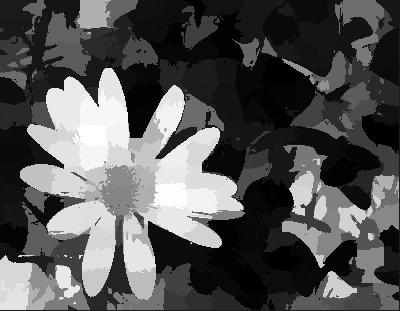
\includegraphics[width=0.3\textwidth,height=0.2\textwidth]{pictures/10841/COLORSALIENCY.jpg} }}%
    \caption{Construction of Color Saliency}%
    \label{fig:conversion23}%
\end{figure}


\section{Final Saliency Map}
Based on the three above mentioned saliency measurements we define the final saliency of a region r\textsubscript{i}, where Sal(ri) is normalized to the range [0,1] afterwards. For combining each map is given different level of  priority to gain better result. Equation \eqref{21} is used to compute the final saliency.



\begin{equation}\label{21}
Sal(r\textsubscript{i}) &=S\textsubscript{B}(r\textsubscript{i})\times W\textsubscript{B}+ S\textsubscript{G}(r\textsubscript{i}) \times W\textsubscript{G}+ S\textsubscript{C}(r\textsubscript{i}) \times W\textsubscript{C}
\end{equation}




\begin{figure}[here]%
    \centering
    \subfloat[Final Saliency Map 
    without smoothing]{{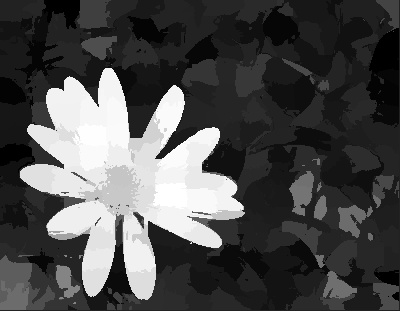
\includegraphics[width=0.45\textwidth,height=0.3\textwidth]{pictures/10841/FinalsaliencyMapWithoutSmoothing.jpg} }}%
    \qquad
    \subfloat[Final Saliency Map 
    with smoothing]{{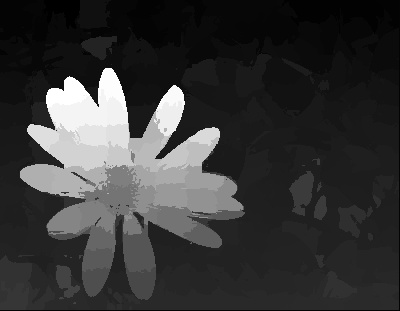
\includegraphics[width=0.45\textwidth,height=0.3\textwidth]{pictures/10841/FinalsaliencyMapWithSmoothing.jpg} }}%
    \caption{Generated final saliency map}%
    \label{superpixel}%
\end{figure}
\noindent
Here W\textsubscript{B}, W\textsubscript{G} and W\textsubscript{C} are different weights to adjust different saliency maps importance.
the output of equation \eqref{21} is then normalized to the range [0,1]

Our final workflow is shown in figure:3.9 
As we can see in the flowchart first an image is taken as input then it is divided into segments. Before dividing it from input image a color importance map is also calculated.
\begin{figure}[here]
  \centering
  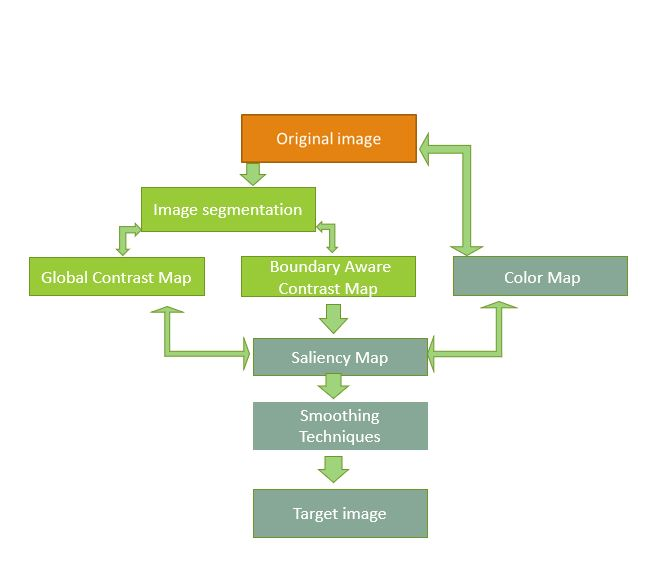
\includegraphics[width=0.7\textwidth,height=0.9\textwidth]{pictures/flowchart.jpg}
  \caption{Flow Diagram of The Process}
  \label{orangeleaf}
\end{figure}

\noindent
Now from the segmented image Global contrast map is calculated and Boundary aware contrast map is also calculated. Then combining these two maps along with the previously built color importance map gives us the saliecy map. We then apply some smoothing technique to make our result better. Then after applying smoothing technique our final output image is generated.



\chapter{Experimental Result}
\section{Introduction}
The evaluation of a predicted foreground map against a
ground-truth (GT) annotation map is crucial in evaluating
and comparing various computer vision algorithm for applications such as object detection\cite{borji2015salient,bylinskii2015saliency,kanan2010robust,qi2015saliencyrank} , saliency
prediction \cite{borji2014salient,hou2017deeply,jiang2013salient}, image segmentation and image collection browsing . As a
specific example, here we focus on salient object detection
models, although the proposed measure is general and can be used for other purposes. It is necessary to point out that the salient object is not necessary to be foreground object \cite{feng2016local}.

\section{Experimental Setup}

The experiments and related analysis are done in this chapter.It gives an assumption of the computation cost of finding visual saliency as well as a benchmark for comparing it to other existing method to find it's advantage and disadvantage. 
The experiments and analysis processes are done on a computer with Core-I3 processor having 2 cores with each core having 1.7GHz Speed. Also the system had 4GB of RAM, and 2 GB of intel hd video memory.
For software, Visual Studio 2015 Professional Edition is used and program is done with C++ language with OpenCV. OpenCV(Open Source Computer Vision) is a library of programming functions mainly aimed at real-time computer vision. It is developed by Intel’s research center at first and later maintained by Willow Garage and now is maintained by Itseez.
The reason for using OpenCV because it gives easy functionality to do different processes without going into implementations. Moreover it gives the benefit to use GPU by which processes can be made faster than using CPU only for computation works.

\subsection{Measuring Terms}

Saliency detection models often generate non-binary
maps. Traditional evaluation measures usually convert
these non-binary maps into multiple binary maps
\subsubsection{Evaluation of binary maps}

To evaluate a binary map,
four values are computed from the prediction confusion matrix: True Positives (TP), True Negatives (TN), False Positives (FP) and False Negatives (FN). These values are then
used to compute three ratios: True Positive Rate (TPR) or
Recall, False Positive Rate (FPR), and Precision.
To find these measures, 4 parameters are required to be known. They are described below:

\begin{enumerate}

\item True Positive: If predicted class is positive and the actual class is also positive then it is called True Positive.
\item True Negative: If predicted class is negative and the actual class is also negative then it is called True Negative.
\item False Positive: If predicted class is positive but the actual class is negative then it is called False Positive.
\item False Negative: If predicted class is negative but the actual class is positive then it is called False Negative.
\end{enumerate}
For example, if there 5 objects, 3 of them are actually Positive, 2 of them are actually negative, but 4 of them are predicted as Positive and 1 of them as negative them no of True Positive is 3, no of True Negative is 1, no of False Positive is 1 and no of False Negative 0.
Accuracy Accuracy is a measure that tells how much accurate the result is. It is expressed as such

\begin{align*}
 Accuracy&= \frac{TruePositive + TrueNegative}{TruePositive + TrueNegative + FalsePositive + FalseNegative}\\
 \end{align*}
\noindent
So accuracy is actually the ratio of the no of objects that are correctly classified divided by the total no of objects. For example, 50 percent accu- racy means 50 out of 100 data objects are correctly classified.
Precision Precision gives a measure that tells how much data objects are correctly and positively classified out of the all positively predicted data objects.

\begin{align*}
Precision &= \frac{TruePositive}{TruePositive + FalsePositive}\\
 \end{align*}
 So if precision is 25 percent,that means 25 data objects are correctly and positively classified out of 100 data objects that are predicted positively.
Recall Recall gives a measure that tells how much data objects are cor- rectly and positively classified out of the all actually positive data objects. It is expressed as such
\begin{align*}
Recall&=\frac{TruePositive}{TruePositive + FalseNegative}\\
 \end{align*} 
So if recall is 75 percent, that means 75 data objects are classified as Posi- tive out of 100 actually positive data objects. This measures give a positive feedback about the outcome, which means the more the values of these measures, the better the outcome is. But these measures might affect to each other. For example, increasing the amount of recall may cause decrease of precision because to increase recall, some portion of the non-foreground might come to the output as foreground, which can decrease the precision.

\subsubsection{Evaluation of non-binary maps}
PR- curve is
universally-agreed evaluation measures. Algorithms that
produce non-binary maps apply three steps to evaluate the agreement between model predictions (non-binary maps)
and human annotations (GT). First, multiple thresholds are
applied to the non-binary map to get multiple binary maps.
Second, these binary maps are compared to the binary mask
of the GT to get a set of TPR(True Positive Rate) & FPR(False Positive Rate) values. These values
are plotted in a 2D plot to get the PR curve.

\subsection{Dataset}
The  MSRA Salient Object Database \cite{cheng2015global}\cite{SalObjSurvey}\cite{SalObjBenchmark}\cite{13iccv/Cheng_Saliency}, which originally provides salient object annotation in terms of bounding boxes provided by 3-9 users, is widely used in salient object detection and segmentation community. Although an invaluable recourse to evaluate saliency detection algorithms, the database with the marked bounding boxes, however, is often too coarse for fine grained evaluation as observed by Wang and Li  \cite{wang2008two}and Achanta et al.\cite{achanta2010saliency}. In order to do more extensive and accurate evaluation, we randomly selected 10,000 images with consistent bounding box labeling in MSRA database. We call this dataset MSRA10K because it contains 10,000 images with pixel-level saliency labeling for 10K images from MSRA dataset.

\begin{figure}%
    \centering
    \subfloat[]{{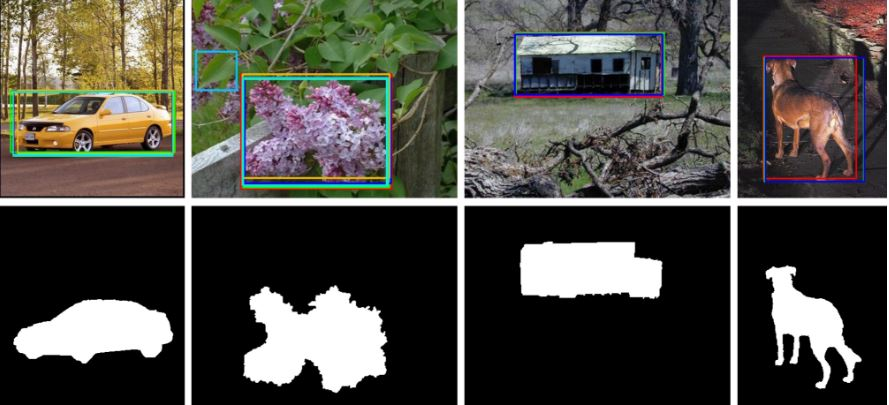
\includegraphics[width=0.6\textwidth,height=0.3\textwidth]{pictures/experiment/data1.jpg} }}%
    \caption{MSRA10k Dataset with Ground Truth and Original Image}%
    \label{fig:conversion23}%
\end{figure}


\subsection{Precision-Recall Curve}
For a saliency map S, we can
convert it to a binary mask M and compute P recision
and Recall by comparing M with ground-truth G.
The binarization
of S is the key step in the evaluation. Usually, there are
three popular ways to perform the binarization. In the first
solution, Achanta et al.\cite{achanta2010saliency} proposed the image-dependent
adaptive threshold for binarizing S, which is computed as
twice as the mean saliency of S.The second way to bipartite S is to use a fixed threshold
which changes from 0 to 255. On each threshold, a pair of precision/recall scores are computed, and are finally
combined to form a precision-recall (PR) curve to describe
the model performance at different situations.
The third way of binarization is to use the SaliencyCut
algorithm \cite{ren2014salient}. In this solution, a loose threshold, which
typically results in good recall but relatively poor precision,
is used to generate the initial binary mask. Then the method
iteratively uses the GrabCut segmentation method\cite{rother2004grabcut} to
gradually refines the binary mask. The final binary mask is
used to re-compute the precision-recall value.
We use the second way or Fixed-thresholding to measure the precision and recall.

\begin{figure}[here]%
    \centering
    \subfloat[]{{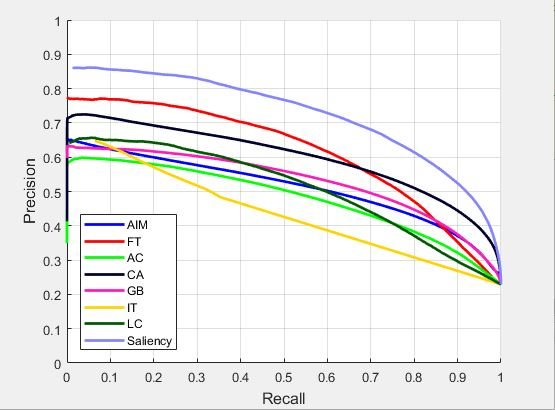
\includegraphics[width=0.7\textwidth,height=0.3\textwidth]{pictures/experiment/data.jpg} }}%
    \caption{Comparison with other method}%
    \label{fig:conversion23}%
\end{figure}
\noindent
From the figure it can be shown that saliency is way higher than other method IT\cite{itti1998model},GB\cite{harel2007graph},LC\cite{zhai2006visual},FT\cite{achanta2009frequency},AIM\cite{bruce2009saliency},CA\cite{goferman2012context}

\subsection{Mean Absolute Error}
The overlap-based
evaluation measures introduced like precision recall curve do not consider the
true negative saliency assignments, i.e., the pixels correctly
marked as non-salient. This favors methods that successfully assign saliency to salient pixels but fail to detect
non-salient regions over methods that successfully detect
non-salient pixels but make mistakes in determining the
salient ones. For a more comprehensive comparison we therefore
also evaluate the mean absolute error (MAE) between the
continuous saliency map S and the binary ground truth G,
both normalized in the range [0, 1]. The MAE score is
defined as:
\noindent
 
\begin{equation}\label{1}
MAE &= \frac{1}{W\times H} \sum_{x=1}^{W} \sum_{y=1}^{H}|S(x,y)-G(x,y)|
\end{equation}

\noindent
Here W is the width of the image and H is the height of the image. Following equation \ref{3} we get the MAE score as follows:
\begin{figure}[here]%
    \centering
    \subfloat[]{{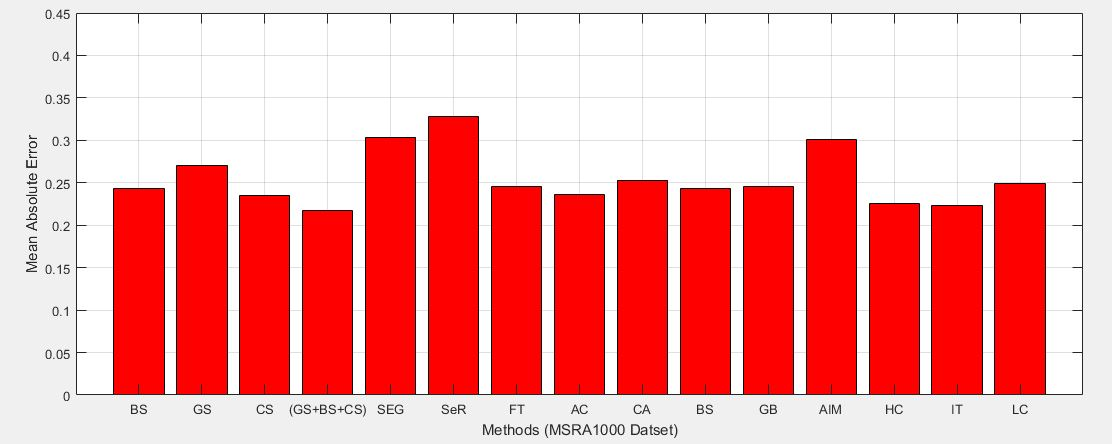
\includegraphics[width=1\textwidth,height=0.4\textwidth]{pictures/experiment/MSRAMAE.jpg} }}%
    \caption{Mean absolute error for MSRA1000 dataset}%
    \label{fig:conversion23}%
\end{figure}
\noindent


We can see that our saliency map combined of color saliency,boundary based saliency and global saliency has low MAE than other existing methods.


\chapter{Conclusion}
\section{Summary}
We propose a simple approach for visually salient region detection effectively where we use color differences between regions as well as spatial distance. Then for making the result more close to ground truth we introduce color importance.
After comparing color difference along with spatial distance between regions visually salient regions are highlighted.Then when comparing each region with boundary regions relatively less visually salient regions which are meant to be background are suppressed. Then when incorporating color importance , we find the mean color of the image and subtract that mean color from every region. We know backgrounds of an image tends to cover more area than foreground. So the mean color will be close to background region and subtraction will eventually suppress the background. We then combine global saliency map, boundary aware contrast map and color importance map to produce our final saliecy map. For generating superpixels we used SLIC which is a fast and convenient algorithm to generate superpixels effectively. We used The  MSRA Salient Object Database \cite{cheng2015global}\cite{SalObjSurvey}\cite{SalObjBenchmark}\cite{13iccv/Cheng_Saliency} to build output and generated precision recall curve to compare the output with ground truth statistically rather than doing it with visual perception.
\section{Limitation}
Some challenges are still needed to be taken into account. For example if part of an object has the same color as background then creating global contrast map,boundary aware contrast map and color importance map  won't be enough to detect that portion. Eventually we will end up with foreground object where the part of it which matched the background will be considered as background. This method is fast, simple yet effective approach to find visually salient regions from images
having simple background. however images having more complex background will fail to produce impressive result using this method. If the border has a frame with same color as foreground object then boundary aware contrast map doesn't contribute at all to detect visually salient region instead it push the output to a negative extent. For images with relatively simple background and foreground this method works fine.



\section{Future Scope}
In the future, we will study more on complex data set, as the data set eliminating center bias. This will make huge challenge to the existing saliency detection methods, may even open up a new research direction of saliency detection.
We will also try to eliminate  our limitations. As this is a preprocessing task of many computer vision related job, the more accurate it gets the result of those computer vision related jobs will also become more accurate.
\noindent
An important need of a robot is to know where it is located. For this aim, the robot can use the data from its sensors to find landmarks (salient features extraction) and register images taken at different times (salient features comparison) to build a model of the scene. The general process of real-time building of a view of the scene is called Simultaneous Localization and Mapping (SLAM). Saliency models can help a lot in the extraction of more stable landmarks from images which can be more robustly compared \cite{frintrop2008attentional}. Those techniques imply first the computation of saliency maps, but the results are not used directly: they need to be further processed (especially comparisons of salient areas).
Another important need of robots after they establish the scene, is to recognize the objects which are present in this scene and which might be interesting to interact with. Two steps are needed to recognize objects. First of all, the robot needs to detect the object in a scene. For this goal saliency models can help a lot as they can provide information about proto-objects or areas objectness . When objects are detected, they need to be recognized.
Among the different applications of automatic saliency computation, the marketing and communication optimization is probably one of the closest to market. As it is possible to predict an image attention map, which is a map of the probability that people attend each pixel of the image, it is possible to predict where people are likely to look on a marketing material like an advertisement or a website. Attracting customer attention is the first step of the process of attracting people interest, induce desire and need for the product and finally push the client to buy it.


\bibliographystyle{unsrt}
\bibliography{ref}

\end{document}